\chapter{Resultados}

Neste capítulo é apresenta a ferramenta obtida assim como detalhes sobre o tempo de execução.


\section[Parte Gráfica]{Parte Gráfica}

A parte gráfica da ferramenta é baseada em duas telas, a tela de exibição que se assemelha a um player e é responsavel exclusivamente para exibir o video e suas modificações e o painel de controle que é destacada do player porem sua unica função é controllar o que será exibido no player.


\begin{figure}[!htb]
	\centering
	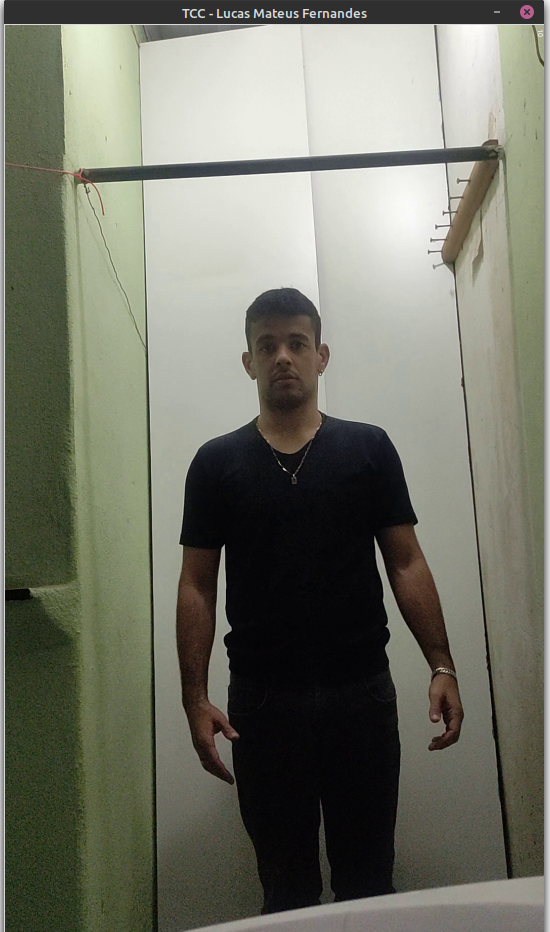
\includegraphics[scale=0.25]{figuras/view/player.png}
	\caption{Tela ``player''}
\end{figure}


A tela responsavel por ser um painel de controle do player possui nove campos de entrada sendo  2 caixas de texto  "Speed" e "Frame" e cinco botões "PLAY", "SaveF", "SaveV", "Barra", "Dados" e "EPH" e uma barra deslizante. 


\begin{figure}[!htb]
	\centering
	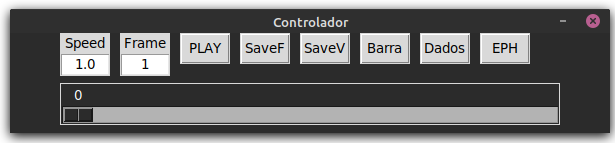
\includegraphics[scale=0.5]{figuras/view/painel_controller.png}
	\caption{Tela ``painel de controle''}
\end{figure}

A caixade texto "Speed" recebe como entrada um numero decimal que representa um scalar pelo qual a velocidade de reproduçaõ vai ser alterada. A caixade texto "Frame" recebe como entrada um numero inteiro e faz com que o video se mova para o \textit{frame} semelhante a barra deslizante que altera o frame em exibição. O botão "PLAY" é responsavel por reproduzir o video e pausar. O botão "SaveF" é responsavel por salvar o frame visualizado no diretorio ./midia/dist do projeto analogamente o botão "SaveV" faz o mesmo porem para um video e não uma imagem. O botão "Barra" é responsavel por  destacar a posição da barra no video. O botão "EPH" é responsavel por destacar a pose do executor traçando segmento de retas sobre os membros e o tronco. O botão "Dados" é responsavel por exibir no canto esquerdo superior informações como  
 id do frame, o estado do \ac{AFD} a quantidade de barras realizada, o angulo entre o braço e ante braço, o angulo formado pela perna e coxa, o angulo pelo qual o video teve que ser rotacionado para a barra ficar paralela ao solo, condiçoes como, se a mão esta tocando a barra se o cotovelo esta extendido ou flexionado se as pernas estão dobradas, se a cabeça ultrapassou a barra, a distancia do peito até a barra, se o peito tocou a barra e o caracter do \ac{AFD} que representa o frame atual.


\begin{figure}[!htb]
	\centering
	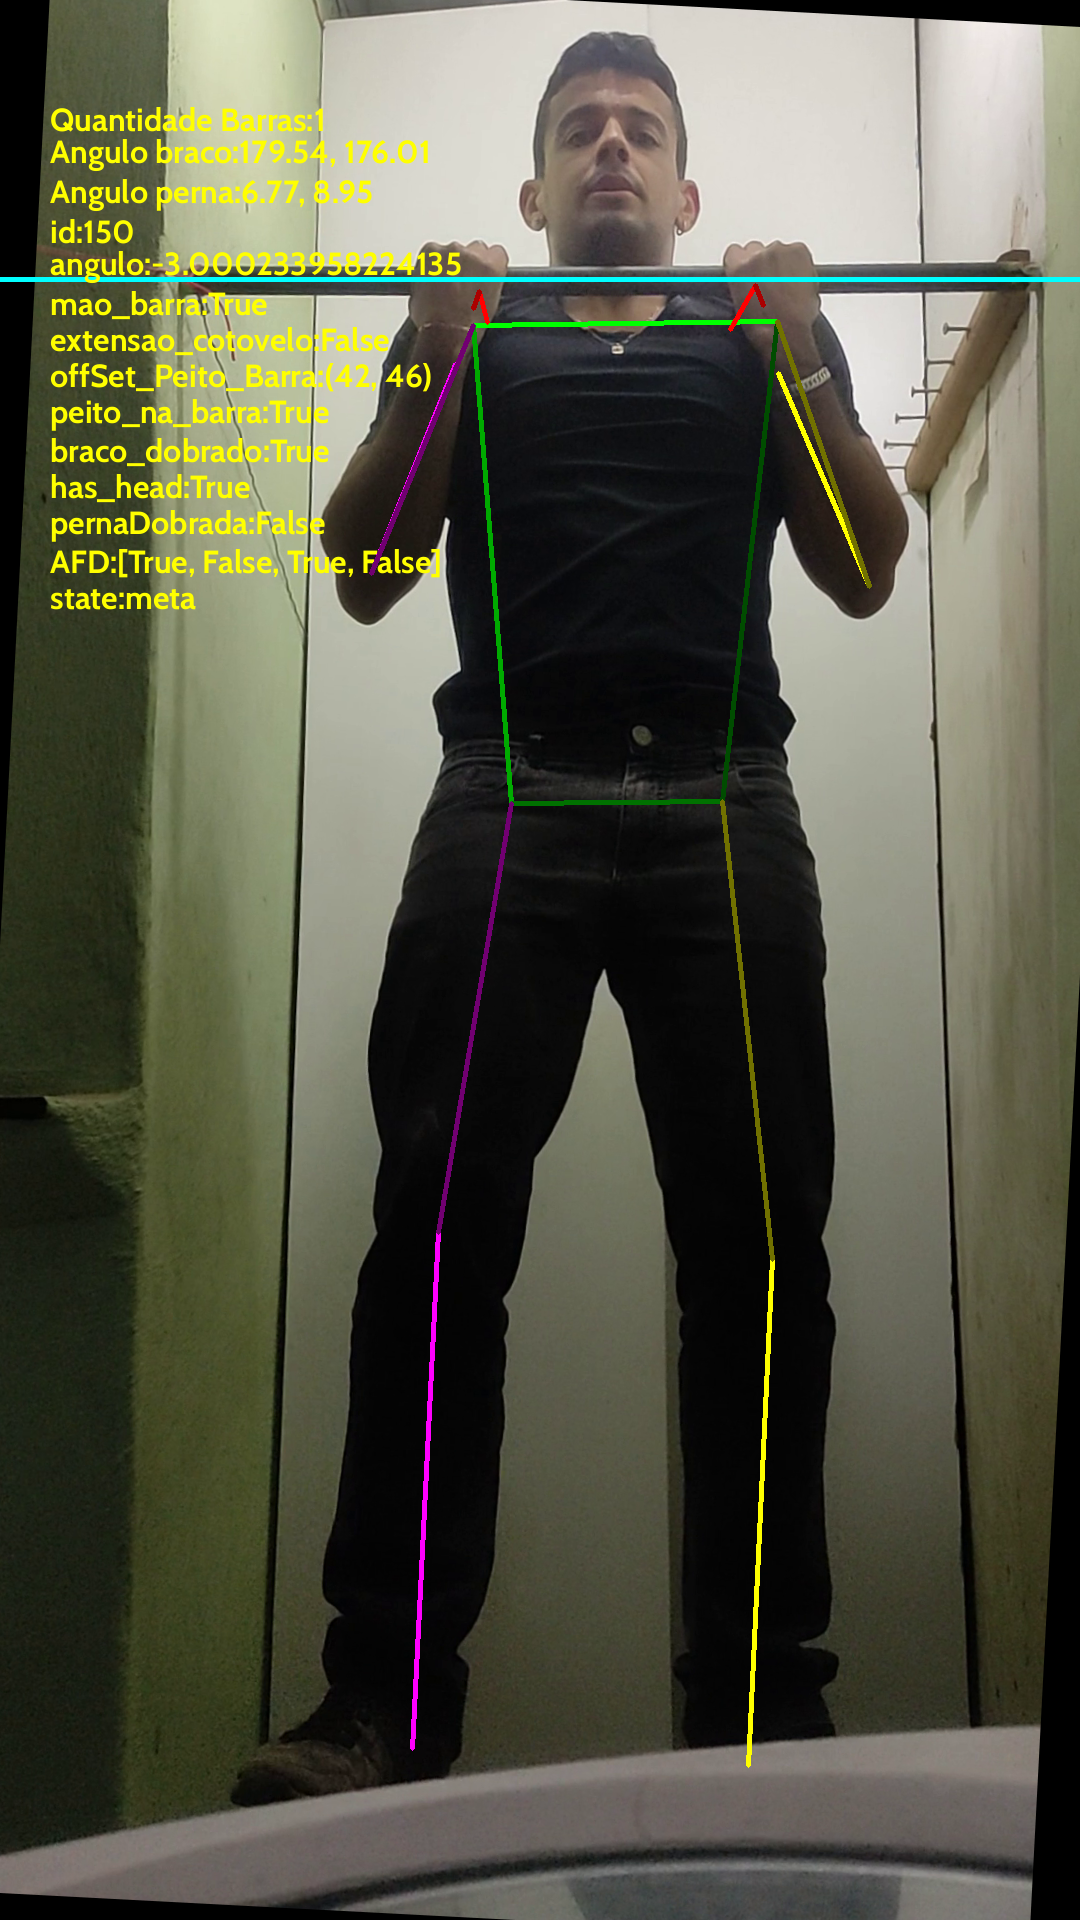
\includegraphics[scale=0.33]{figuras/flags.png}
	\caption{Resultado final com todas as Flags ativas ``Barra'',``Dados'' e ``EPH''}
\end{figure}
\newpage



\section[Tempo de execução]{Tempo de execução}

O tempo de execução desempenha um papel crucial pois representa o intervalo de tempo necessário para que um programa ou algoritmo conclua uma tarefa específica e é um fator fundamental na avaliação e otimização de sistemas computacionais utilizado como métrica para comparar a eficiência de diferentes abordagens e soluções, buscando identificar a estratégia mais eficaz para realizar uma tarefa determinada.Portanto para os testes foi avaliado um video de 211 frames a uma taxa de 24 frames por segundos realizando um execução correta do movimento de barra fixa, para a amostragem foi realizado 10 iterações da execução o programa.


 
A função 'barra' é responsável pela identificação da barra, conforme demonstrado em \ref{sec:Deteccao da barra}. O gráfico abaixo mostra o tempo gasto em segundos pela função 'barra' no eixo vertical e associa esse tempo ao identificador do frame no eixo horizontal. O tempo médio para essa operação foi de 0,03422 segundos, enquanto o menor tempo registrado foi de 0,016335 segundos.

\begin{figure}[!htb]
	\centering
	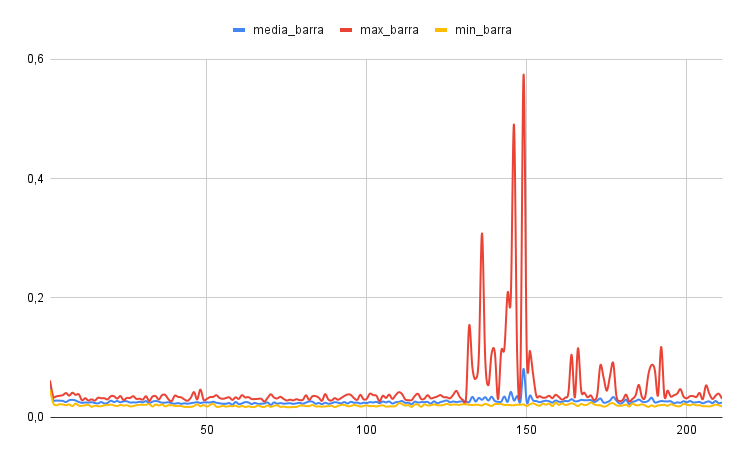
\includegraphics[scale=0.6]{figuras/grafico/barra.png}
	\caption{Tempo de execução da função 'barra' em 10 iterações mostrando a média, mínimo e máximo do tempo gasto por quadro em segundos}
\end{figure}


A função 'verify\_inclination' é responsável pela rotação da imagem de acordo com a rotação da barra, conforme demonstrado em \ref{sec:Inclinacao da barra}. O gráfico abaixo mostra o tempo gasto em segundos pela função 'verify\_inclination' no eixo vertical e associa esse tempo ao identificador do frame no eixo horizontal. O tempo médio para essa operação foi de 0,00603 segundos, enquanto o menor tempo registrado foi de 0,00317 segundos.

\begin{figure}[!htb]
	\centering
	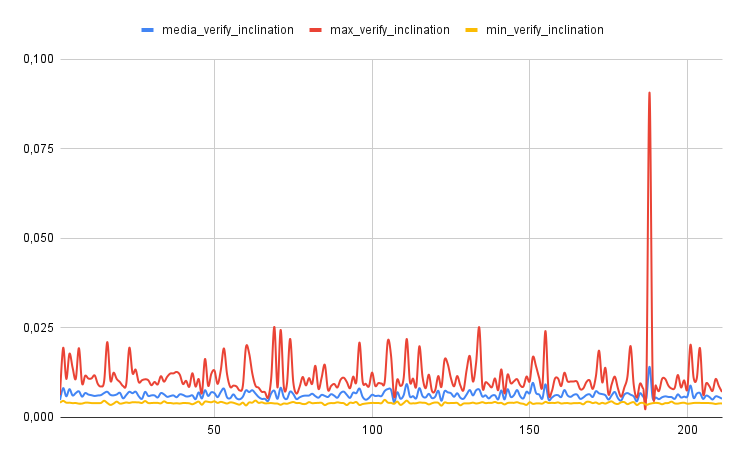
\includegraphics[scale=0.6]{figuras/grafico/inclination.png}
	\caption{Tempo de execução da função 'verify\_inclination' em 10 iterações mostrando a média, mínimo e máximo do tempo gasto por quadro em segundos}
\end{figure}





A função 'verify\_eph' é responsável pela identificação dos pontos chaves do corpo humano, conforme demonstrado em \ref{sec:Reconhecimento de pose humana}. O gráfico abaixo mostra o tempo gasto em segundos pela função 'verify\_eph' no eixo vertical e associa esse tempo ao identificador do frame no eixo horizontal. O tempo médio para essa operação foi de 0,1293617 segundos, enquanto o menor tempo registrado foi de 0,109623 segundos.


\begin{figure}[!htb]
	\centering
	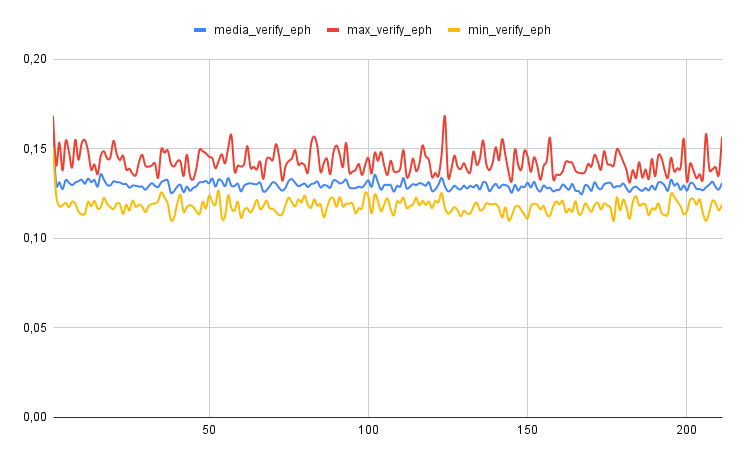
\includegraphics[scale=0.5]{figuras/grafico/eph.png}
	\caption{Tempo de execução da função 'verify\_eph' em 10 iterações mostrando a média, mínimo e máximo do tempo gasto por quadro em segundos}
\end{figure}






A função 'verify\_angle\_member' é responsável pela identificação dos angulos entre os segmentos, conforme demonstrado em \ref{angulo_braco} e \ref{sec:quadril}. O gráfico abaixo mostra o tempo gasto em segundos pela função 'verify\_angle\_member' no eixo vertical e associa esse tempo ao identificador do frame no eixo horizontal. O tempo médio para essa operação foi de 0,00013 segundos, enquanto o menor tempo registrado foi de 0,000045 segundos.

\begin{figure}[!htb]
	\centering
	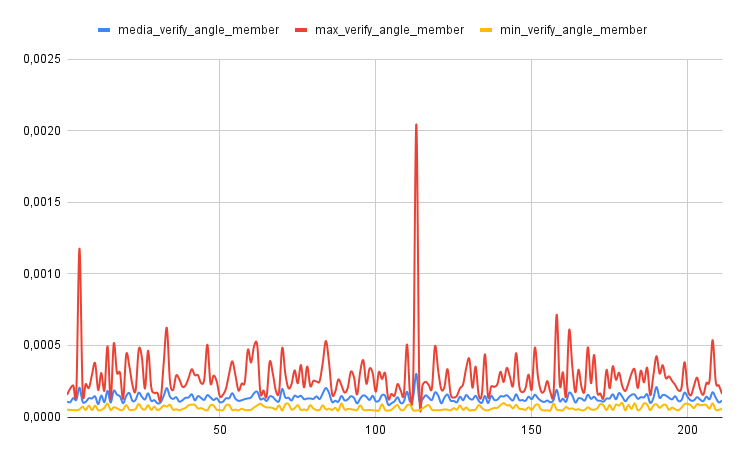
\includegraphics[scale=0.6]{figuras/grafico/angulo.png}
	\caption{Tempo de execução da função 'verify\_angle\_member' em 10 iterações mostrando a média, mínimo e máximo do tempo gasto por quadro em segundos}
\end{figure}




\begin{sloppypar}
    A função 'verify\_char\_AFD' é um compilado de 4 funções sendo elas 'verify\_maoBarra' \ref{sec:Mao na barra}, 'verify\_extensaoCotovelo' \ref{sec:Braco esticado}, 'verify\_ultrapassarBarra' \ref{sec:meta} e 'verify\_movimentoQuadrilPerna' \ref{sec:quadril} responsaveis pela extração da informação presente no caracter do \ac{AFD} \ref{lst:caracter}. O gráfico abaixo mostra o tempo gasto em segundos pela função 'verify\_char\_AFD' no eixo vertical e associa esse tempo ao identificador do frame no eixo horizontal. O tempo médio para essa operação foi de 0,0753571 segundos, enquanto o menor tempo registrado foi de 0,039386 segundos.Sendo que o componente mais significato em sua execução foi 'verify\_maoBarra' 
\end{sloppypar}


\begin{figure}[!htb]
	\centering
	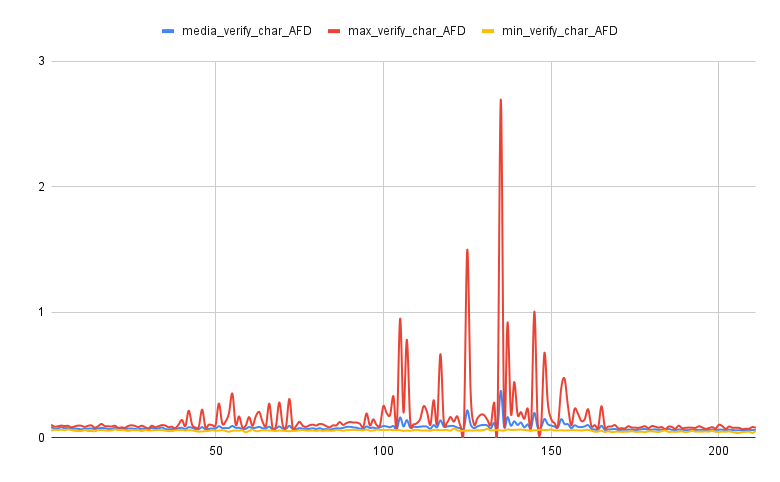
\includegraphics[scale=0.55]{figuras/grafico/char_AFD.png}
	\caption{Tempo de execução da função 'verify\_char\_AFD' em 10 iterações mostrando a média, mínimo e máximo do tempo gasto por quadro em segundos}
\end{figure}

\begin{figure}[!htb]
	\centering
	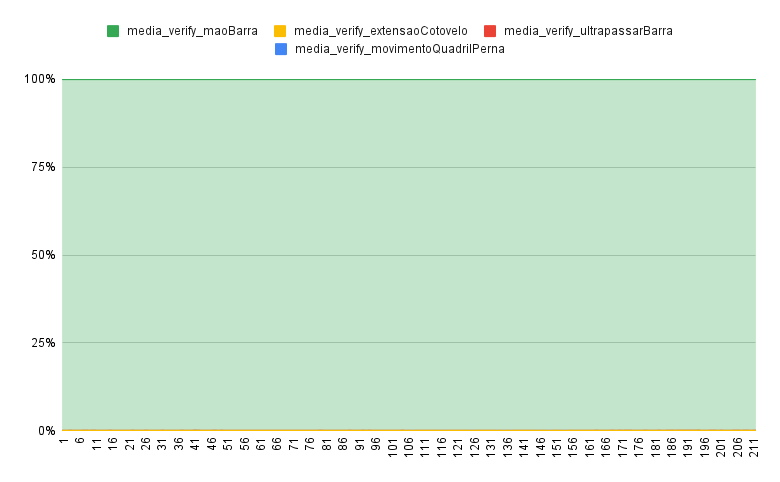
\includegraphics[scale=0.55]{figuras/grafico/comp_char_AFD.png}
	\caption{Composição da função 'verify\_char\_AFD' em 10 iterações mostrando o tempo médio de cada componente em relação a  'verify\_char\_AFD' }
\end{figure}

\newpage

Os gráficos abaixo mostram o tempo gasto em segundos pelas funçoes que compõe a função 'verify\_char\_AFD' sendo que no eixo vertical é descriminado o tempo em segundos e no eixo 
 horizontal o identificador do frame.

\begin{figure}[!htb]
	\centering
	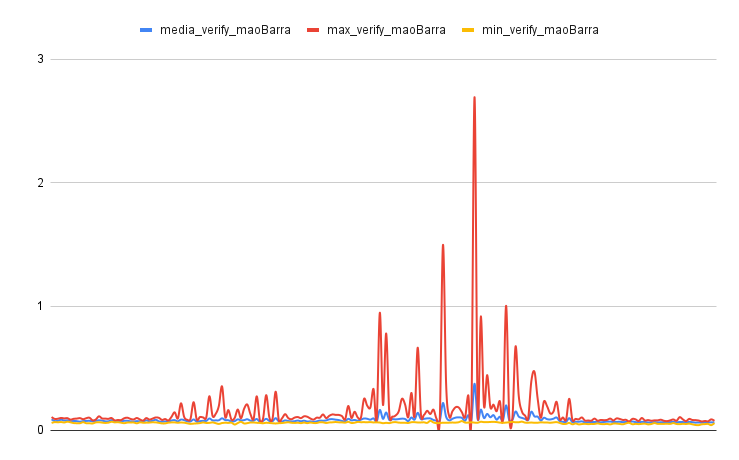
\includegraphics[scale=0.6]{figuras/grafico/maoBarra.png}
	\caption{Tempo de execução da função 'verify\_maoBarra' em 10 iterações mostrando a média, mínimo e máximo do tempo gasto por quadro em segundos}
\end{figure}

\begin{figure}[!htb]
	\centering
	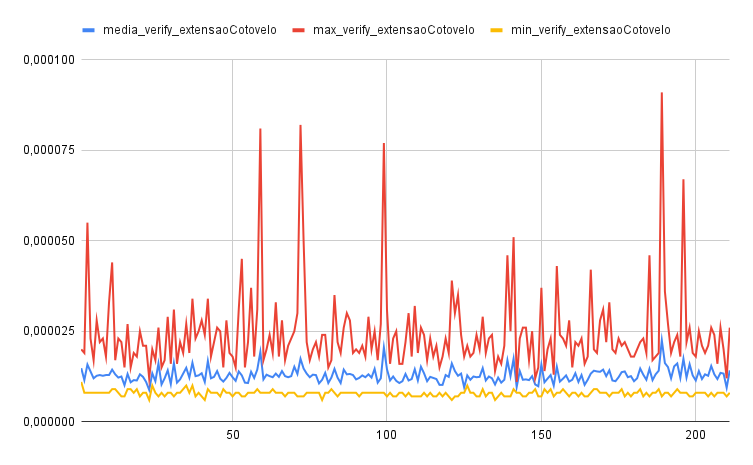
\includegraphics[scale=0.6]{figuras/grafico/extensaoCotovelo.png}
	\caption{Tempo de execução da função 'verify\_extensaoCotovelo' em 10 iterações mostrando a média, mínimo e máximo do tempo gasto por quadro em segundos}
\end{figure}

\begin{figure}[!htb]
	\centering
	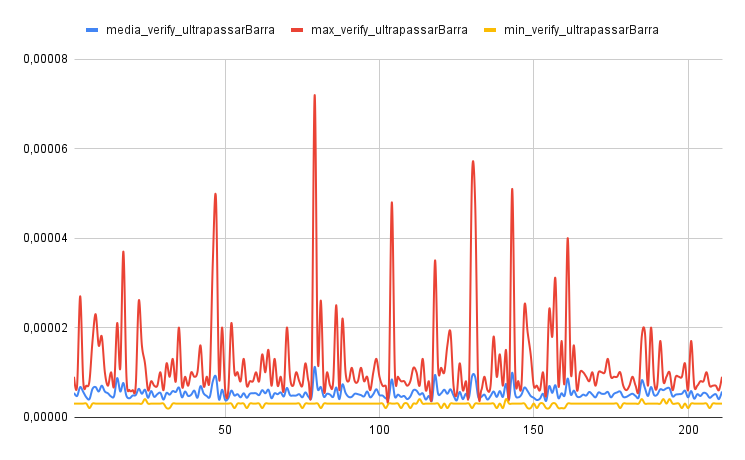
\includegraphics[scale=0.6]{figuras/grafico/ultrapassarBarra.png}
	\caption{Tempo de execução da função 'verify\_ultrapassarBarra' em 10 iterações mostrando a média, mínimo e máximo do tempo gasto por quadro em segundos}
\end{figure}

\begin{figure}[!htb]
	\centering
	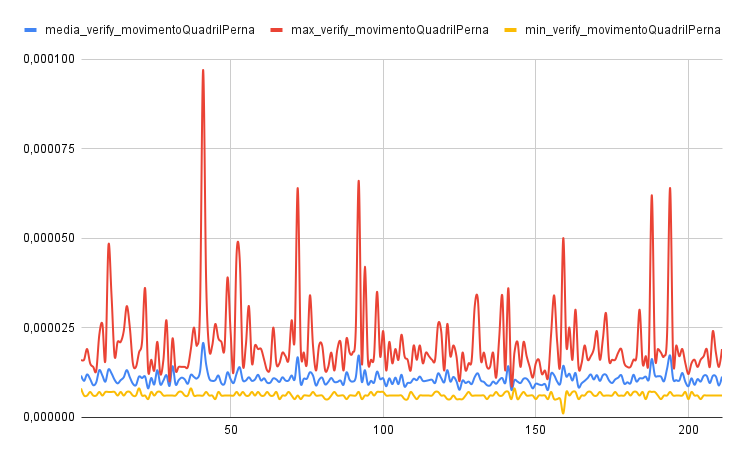
\includegraphics[scale=0.6]{figuras/grafico/movimentoQuadril.png}
	\caption{Tempo de execução da função 'verify\_movimentoQuadrilPerna' em 10 iterações mostrando a média, mínimo e máximo do tempo gasto por quadro em segundos}
\end{figure}

.
\newpage

A função 'verify\_maoBarra' teve um tempo médio de 0,0747025 segundos, enquanto o menor tempo registrado foi de 0,03924 segundos e o maior tempo alcançado entre a media das 10 iterações foi de 0,3741517 segundos. A função 'verify\_extensaoCotovelo' teve um tempo médio de 0,0000126 segundos, enquanto o menor tempo registrado foi de 0,000006 segundos.A função 'verify\_ultrapassarBarra' teve um tempo médio de0,0000051 segundos, enquanto o menor tempo registrado foi de 0,000002 segundos. A função 'verify\_movimentoQuadrilPerna' teve um tempo médio de 0,0000104 segundos, enquanto o menor tempo registrado foi de 0,000001 segundos.



A função 'verify\_AFD' é responsavel pela computação do \ac{AFD} \ref{fig:transicaoAFD}. O gráfico abaixo mostra o tempo gasto em segundos pela função 'verify\_AFD' no eixo vertical e associa esse tempo ao identificador do frame no eixo horizontal. O tempo médio para essa operação foi de 0,0000427 segundos, enquanto o menor tempo registrado foi de 0,000016 segundos.

\begin{figure}[!htb]
	\centering
	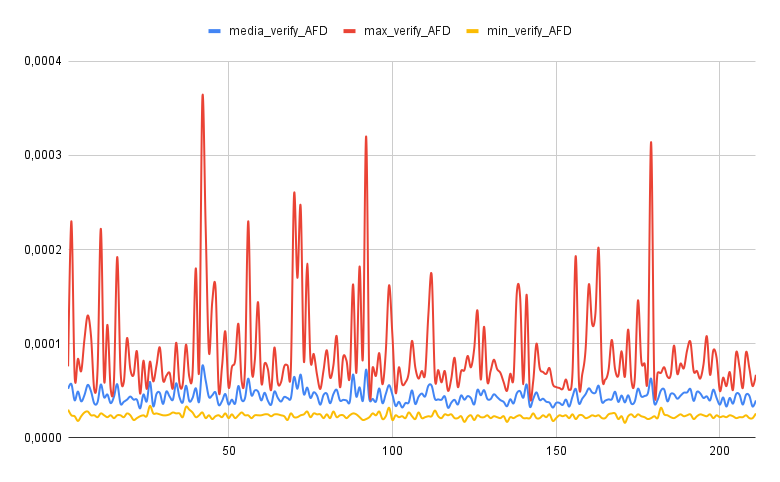
\includegraphics[scale=0.55]{figuras/grafico/verify_AFD.png}
	\caption{Tempo de execução da função 'verify\_AFD' em 10 iterações mostrando a média, mínimo e máximo do tempo gasto por quadro em segundos}
\end{figure}


Por fim todas essas funções são englobadas dentro da função 'process\_cell'. O gráfico abaixo mostra o tempo gasto em segundos pela função 'process\_cell' no eixo vertical e associa esse tempo ao identificador do frame no eixo horizontal. O tempo médio para essa operação foi de 0,2403654 segundos, enquanto o menor tempo registrado foi de 0,171841 segundos. 

\begin{figure}[!htb]
	\centering
	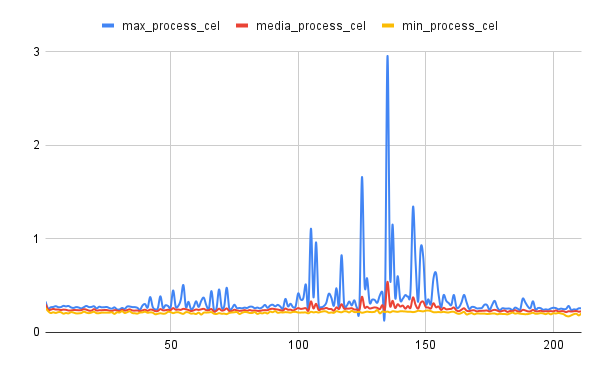
\includegraphics[scale=0.6]{figuras/grafico/process_cell.png}
	\caption{Tempo de execução da função 'process\_cell' em 10 iterações mostrando a média, mínimo e máximo do tempo gasto por quadro em segundos}
\end{figure}

\begin{figure}[!htb]
	\centering
	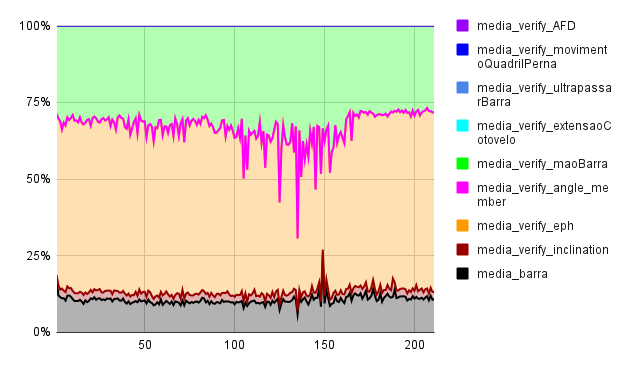
\includegraphics[scale=0.6]{figuras/grafico/comp_process_cell_1.png}
	\caption{Tempo medio de 10 iterações das funções que compõe 'process\_cell' em segundos}
\end{figure}

\begin{figure}[!htb]
	\centering
	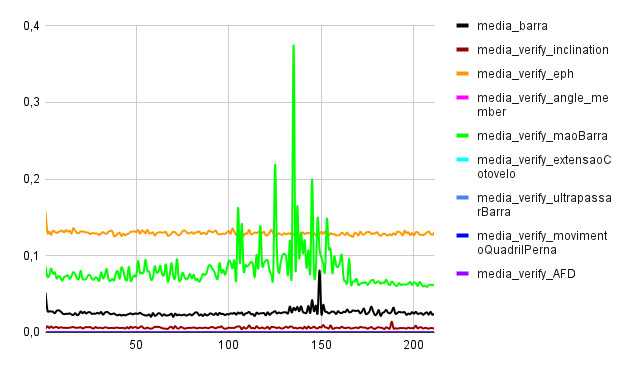
\includegraphics[scale=0.6]{figuras/grafico/comp_process_cell_2.png}
	\caption{Composição da função 'process\_cell' em 10 iterações mostrando o tempo médio de cada componente em relação a  'process\_cell' }
\end{figure}

\newpage
As 2 funções mais relevantes para a alta taxa de latência do processamento do frame é responsavel por 'verify\_eph' e 'verify\_maoBarra' responsavel por cerca de 85.14\% do tempo gasto em 'process\_cell'



